\section[I Sistemi]{I Sistemi}
\sectionframe{images/covers/cover_intro.jpg}{Intro}

\subsection[Intro]{Intro}

% Pastorello: intro_statistical_learning
% https://www.javatpoint.com/machine-learning
\begin{frame}
	\frametitle{Sistema e Stato}
	
	\begin{block}{Sistema}
		Un \textbf{sistema} è un insieme di elementi in relazione tra di loro secondo leggi ben precise che concorrono al raggiungimento di un obiettivo comune.
	\end{block}
	\begin{block}{Stato}
		Il sistema, in base al dati ricevuti in ingresso ed alla sua natura, evolve istante dopo istante in una nuova situazione che è chiamata \textbf{stato}.
	\end{block}
\end{frame}


\begin{frame}
	\frametitle{Esempi di sistemi e stati}
	
	\begin{block}{Esempi di sistemi e stati}
		Potremmo paragonare lo stato di un sistema ad una fotografia del sistema in un dato istante:
		\begin{itemize}
			\item \textbf{Sistema contatore del gas}: in tale contesto lo \textbf{stato} del sistema corrisponde alla cifra dei Smc (standard metro cubo) consumati fino a quell'istante.
			\item \textbf{Sistema distributore automatico delle bibite}: in tale contesto lo \textbf{stato} del sistema corrisponde alle bibite presenti nei vari slot ed al denaro per restituire il resto presente nella macchina.
		\end{itemize}
	\end{block}
\end{frame}


\begin{frame}
	\frametitle{Catalogazione dei sistemi}
	
	\begin{block}{Catalogazione dei sistemi}
		Distinguiamo tra loro vari sistemi separandoli in tre grandi categorie
		\begin{itemize}
			\item \textbf{Sistemi naturali}: per esempio il sistema circolatorio dell’uomo, un albero da frutto.
			\item \textbf{Sistemi artificiali}: per esempio un distributore di bibite o un ascensore
			\item \textbf{Sistemi misti}: per esempio una centrale telefonica.
		\end{itemize}
	\end{block}
\end{frame}


\begin{frame}
	\frametitle{Un qualunque sistema X}
	
	\begin{block}{Potremmo rappresentare qualunque sistema X nel seguente modo:}
		\begin{itemize}
			\item Riceve un insieme di informazioni di partenza \textbf{I} che chiameremo \textbf{inputs}.
			\item Può modificare lo/gli stato/stati \textbf{S} nel quale si può trovare in un determinato istante.
			\item Fornisce un insieme di risposte \textbf{O} che chiameremo \textbf{outputs}.
		\end{itemize}
		
		\begin{figure}[!htbp]
			\centering
			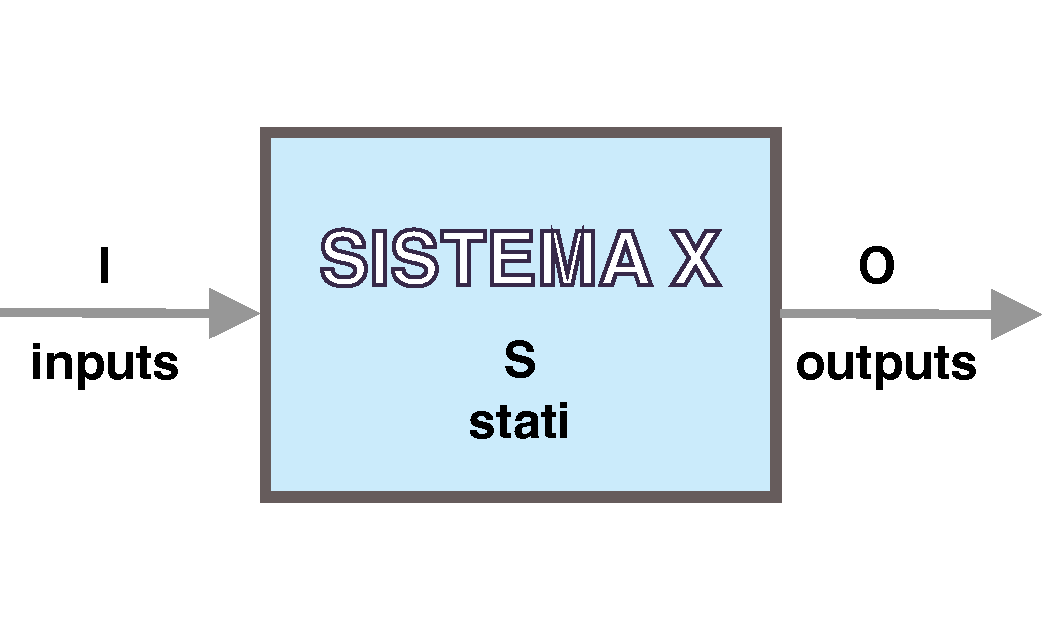
\includegraphics[width=0.45\linewidth]{images/1_i_sistemi/sistemaX.pdf}
					%\caption{}
		\end{figure}
	\end{block}
\end{frame}